\paragraph{QuizziPedia::Back-End::App::Models::UserProModel}
\label{QuizziPedia::Back-End::App::Models::UserProModel}
\begin{figure}
	\centering
	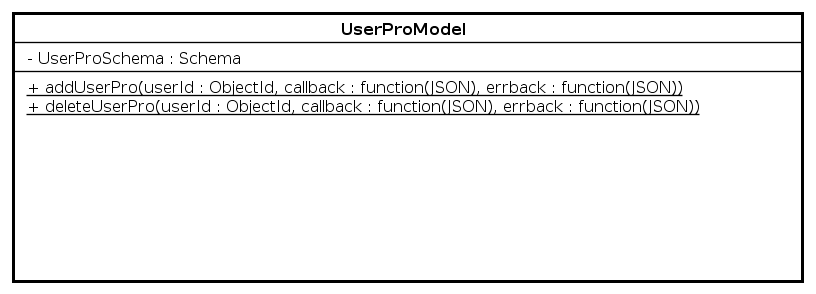
\includegraphics[scale=0.45]{UML/Classi/Back-End/QuizziPedia_Back-End_App_Models_userProModel.png}
	\caption{QuizziPedia::Back-End::App::Models::UserProModel}
\end{figure}
\FloatBarrier
\begin{itemize}
	\item \textbf{Descrizione} \\
	Classe che modella i dati dell'utente pro.
	\item \textbf{Utilizzo} \\
	Viene utilizzata per rappresentare i dati dell'utente pro. Si interfaccia alla libreria Mongoose per la creazione dello schema e dei relativi metodi statici o di istanza.
	\item \textbf{Relazioni con altre classi} 
		\begin{itemize}
			\item IN \textbf {UserManagementController} \\
			Classe che gestisce la logica applicativa riguardante la visualizzazione e la modifica dei dati dell'utente.
Rappresenta il ConcreteHandler nel design pattern Chain of responsibility. Utilizza Passport.
			\item IN \textbf{QuizModel} \\
			Questa classe rappresenta i dati dei questionari creati dagli utenti Pro.
			\item OUT \textbf{UserModel} \\
			Questa classe rappresenta i dati riguardanti i vari utenti registrati al sistema.
		\end{itemize}
	\item \textbf{Attributi} 
		\begin{itemize}
			\item \textbf{- \texttt{UserProSchema}: \texttt{Schema}} \\
			Questo campo dati rappresenta lo schema Mongoose dell'utente pro QuizziPedia. Lo schema prevede i seguenti attributi:
			\begin{itemize}
				\item 
					\texttt{userID} di tipo \texttt{ObjectId}, rappresenta il riferimento all'identificativo nel database contenente i dati dei vari utenti registrati;
			\end{itemize}		
		\end{itemize}	
	\item \textbf{Metodi}
		\begin{itemize}
		\item
		+ \texttt{addUserPro(userId : ObjectId, callback: function(JSON), errback: function(QuizzipediaError))} \\	
		Questo metodo è statico ed aggiorna la tipologia di utenza. In specifico l'utente di tipo basic passerà a pro. Ritorna un JSON contenente i dati del nuovo utente pro, qualora si siano verificati problemi verrà ritornato un messaggio d'errore.	\\	
		\textbf{Parametri} 
			\begin{itemize}
			\item
				\texttt{userId: ObjectId} \\
				Rappresenta l'identificativo dell'utente da passare a pro
			\item	
				\texttt{callback: function(JSON)} \\
				Rappresenta la callback che il metodo deve chiamare al termine dell'elaborazione.	
			\item	
				\texttt{errback: function(QuizzipediaError)} \\
				Questo parametro rappresenta la callback che il metodo deve chiamare qualora si verificassero errori nell'esecuzione del metodo.		
			\end{itemize}	
		\item	
		+ \texttt{deleteUserPro(userId : ObjectId, callback: function(JSON), errback: function(QuizzipediaError))} \\	
		Questo metodo è statico ed aggiorna la tipologia di utenza. In specifico l'utente di tipo pro ritornerà a basic, eliminando il riferimento alla classe user . Ritorna un JSON contenente i dati dell'utente pro ritornato a basic, qualora si siano verificati problemi verrà ritornato un messaggio d'errore.	\\	
		\textbf{Parametri} 
			\begin{itemize}
			\item
				\texttt{userId: ObjectId} \\
				Rappresenta l'identificativo dell'utente pro da ritornare a basic
			\item	
				\texttt{callback: function(JSON)} \\
				Rappresenta la callback che il metodo deve chiamare al termine dell'elaborazione.	
			\item	
				\texttt{errback: function(QuizzipediaError)} \\
				Questo parametro rappresenta la callback che il metodo deve chiamare qualora si verificassero errori nell'esecuzione del metodo.		
			\end{itemize}		
		\end{itemize}
		
\end{itemize}